% ============================================================
%  Đồ án Tốt nghiệp Đại học — ĐHBK Hà Nội
%  Đề tài: Đánh giá hiệu quả HARQ trong mạng 5G NTN
%  Sinh viên: Hoàng Tuấn Dương  |  Năm: 2026
%
%  Compile (3 lần để refs/toc ổn định):
%    xelatex main.tex
%    bibtex  main
%    xelatex main.tex
%    xelatex main.tex
% ============================================================
\documentclass{article}

% ── Font & encoding (XeLaTeX — UTF-8 native, không cần T5) ──────────────
\usepackage{fontspec}
\defaultfontfeatures{Ligatures=TeX}
% Times New Roman nếu có; fallback sang Latin Modern Serif (luôn có trong TeX Live)
\IfFontExistsTF{Times New Roman}{%
    \setmainfont{Times New Roman}%
}{%
    \setmainfont{Latin Modern Roman}%
}

% ── Layout ──────────────────────────────────────────────────────────────
\usepackage[fontsize=13pt]{scrextend}
\usepackage[paperheight=29.7cm,paperwidth=21cm,
            right=2cm,left=3cm,top=2cm,bottom=2.5cm,twoside]{geometry}
\renewcommand{\baselinestretch}{1.2}
\setlength{\parskip}{6pt}
\setlength{\parindent}{1cm}

% ── Math ────────────────────────────────────────────────────────────────
\usepackage{amsmath,amssymb,unicode-math}
\setmathfont{Latin Modern Math}

% ── Graphics & floats ───────────────────────────────────────────────────
\usepackage{graphicx}
\usepackage{float}
\usepackage{tikz}
\usetikzlibrary{calc}
\graphicspath{{../results/figures/}{./}}

% ── Tables ──────────────────────────────────────────────────────────────
\usepackage{booktabs}
\usepackage{multirow}
\usepackage{tabularx}
\usepackage{xcolor}
\usepackage{colortbl}
\definecolor{LightCyan}{rgb}{0.88,1,1}
\newcolumntype{s}{>{\hsize=.3\hsize}X}
\newcolumntype{y}{>{\hsize=.4\hsize}X}
\newcolumntype{a}{>{\hsize=1.1\hsize}X}
\renewcommand{\tabularxcolumn}[1]{>{\small}m{#1}}

% ── Section heading format ───────────────────────────────────────────────
\usepackage{titlesec}
\setcounter{secnumdepth}{4}
\titlespacing*{\section}{0pt}{0pt}{30pt}
\titleformat*{\section}{\fontsize{16pt}{0pt}\selectfont\bfseries\centering}
\titlespacing*{\subsection}{0pt}{6pt}{0pt}
\titleformat*{\subsection}{\fontsize{14pt}{0pt}\selectfont\bfseries}
\titlespacing*{\subsubsection}{0pt}{6pt}{0pt}
\titleformat*{\subsubsection}{\fontsize{13pt}{0pt}\selectfont\bfseries\itshape}
\titlespacing*{\paragraph}{0pt}{0pt}{0pt}
\titleformat*{\paragraph}{\fontsize{13pt}{0pt}\selectfont\itshape}

% ── Captions ────────────────────────────────────────────────────────────
\usepackage{indentfirst}
\usepackage[font=bf]{caption}
\renewcommand{\figurename}{\fontsize{12pt}{0pt}\selectfont\bfseries Hình}
\renewcommand{\thefigure}{\thesection.\arabic{figure}}
\captionsetup[figure]{labelsep=colon,justification=centering,singlelinecheck=false}
\renewcommand{\tablename}{\fontsize{12pt}{0pt}\selectfont\bfseries Bảng}
\renewcommand{\thetable}{\thesection.\arabic{table}}
\captionsetup[table]{labelsep=colon,position=top,justification=centering,singlelinecheck=false}

% ── Equations & theorems ─────────────────────────────────────────────────
\renewcommand{\theequation}{\thesection.\arabic{equation}}
\newtheorem{theorem}{Định lý}[section]
\newtheorem{defn}[theorem]{Định nghĩa}
\newtheorem{corollary}[theorem]{Hệ quả}
\newtheorem{lemma}[theorem]{Bổ đề}

% ── TOC / list names (Vietnamese) ────────────────────────────────────────
\renewcommand{\contentsname}{MỤC LỤC}
\renewcommand{\listfigurename}{DANH MỤC HÌNH VẼ}
\renewcommand{\listtablename}{DANH MỤC BẢNG BIỂU}
\renewcommand{\refname}{TÀI LIỆU THAM KHẢO}

% ── Hyperlinks & lists ───────────────────────────────────────────────────
\usepackage[unicode,hidelinks]{hyperref}
\usepackage{enumitem}
\setitemize{itemsep=0pt,leftmargin=1.25cm,topsep=3pt}

% ============================================================
\begin{document}

\begin{titlepage}
\begin{tikzpicture}[overlay,remember picture]
\draw [line width=3pt]
    ($ (current page.north west) + (3.0cm,-2.0cm) $)
    rectangle
    ($ (current page.south east) + (-2.0cm,2.5cm) $);
\draw [line width=0.5pt]
    ($ (current page.north west) + (3.1cm,-2.1cm) $)
    rectangle
    ($ (current page.south east) + (-2.1cm,2.6cm) $);
\end{tikzpicture}
\begin{center}
\vspace{-12pt}
ĐẠI HỌC BÁCH KHOA HÀ NỘI \\
\textbf{\fontsize{16pt}{0pt}\selectfont TRƯỜNG ĐIỆN -- ĐIỆN TỬ}\\[0.6cm]

\includegraphics[height=4cm,keepaspectratio]{2_bvp_logo_bk_rgb_148177}\\[0.8cm]
\fontsize{20pt}{0pt}\selectfont BÁO CÁO\\
\vspace{8pt}
\textbf{\fontsize{26pt}{0pt}\selectfont BÀI TẬP LỚN}\\
\vspace{6pt}
\fontsize{14pt}{0pt}\selectfont Môn: Thông tin vệ tinh
\vspace{1.2cm}
\end{center}
\hspace{6pt}\textbf{\fontsize{14pt}{0pt}\selectfont Đề tài:}
\begin{center}
    \textbf{\fontsize{18pt}{0pt}\selectfont ĐÁNH GIÁ HIỆU QUẢ CƠ CHẾ HARQ}\\
    \textbf{\fontsize{18pt}{0pt}\selectfont TRONG MẠNG 5G PHI MẶT ĐẤT (NTN)}

\vspace{1.5cm}
\begin{table}[H]
    \centering
    \begin{tabular}{l l}
 \fontsize{14pt}{0pt}\selectfont Sinh viên thực hiện:    & \fontsize{14pt}{0pt}\selectfont VŨ THỊ GẤM \hspace{4pt}-- 20241720E \vspace{6pt} \\
\fontsize{14pt}{0pt}\selectfont Giảng viên hướng dẫn: & \fontsize{14pt}{0pt}\selectfont PGS. TS. Nguyễn Hoàng Hải \vspace{4pt} \\
    & \fontsize{14pt}{0pt}\selectfont PGS. TS. Lâm Hồng Thạch
\end{tabular}
\end{table}
\vspace{3.0cm}
 \fontsize{14pt}{0pt}\selectfont Hà Nội, 06-2026
\end{center}
\end{titlepage}
\cleardoublepage

\section*{LỜI NÓI ĐẦU}
\phantomsection\addcontentsline{toc}{section}{\numberline {}LỜI NÓI ĐẦU}

Đồ án này được thực hiện trong bối cảnh mạng 5G phi mặt đất (NTN) đang trở thành một trong những hướng phát triển trọng tâm của cộng đồng nghiên cứu viễn thông quốc tế. Kể từ khi 3GPP chính thức đưa hỗ trợ NTN vào Release 17 (năm 2022), câu hỏi về khả năng tương thích của các cơ chế giao thức vốn được thiết kế cho mạng mặt đất -- trong đó có HARQ -- với đặc thù độ trễ cao và liên kết LOS mạnh của kênh vệ tinh, trở thành một bài toán mở và có giá trị thực tiễn cao.

Công trình nghiên cứu của Tuninato và cộng sự (2025)~\cite{tuninato2025} là một trong những bài báo đầu tiên phân tích hệ thống sự đánh đổi giữa HARQ và RLC ARQ trong 5G NTN. Đồ án này được xây dựng dựa trên nền tảng đó, mở rộng thêm phân tích theo nhiều chiều: tổng hợp N$_{\min}$ cho bốn quỹ đạo × bốn cấu hình SCS, đánh giá hiệu quả năng lượng trên bit, và xác minh độc lập toàn bộ kết quả số bằng phân tích CDF Rician từ lý thuyết xác suất.

Em xin chân thành cảm ơn giảng viên hướng dẫn đã định hướng và hỗ trợ trong suốt quá trình thực hiện đồ án.

\vspace{12pt}
\begin{flushright}
\textit{Hà Nội, tháng 6 năm 2026}\\
\textit{Sinh viên thực hiện}\\
\vspace{24pt}
\textbf{Hoàng Tuấn Dương}
\end{flushright}
\cleardoublepage


\addtocontents{toc}{\protect\thispagestyle{empty}}
\tableofcontents
\thispagestyle{empty}
\cleardoublepage

\pagenumbering{roman}
\section*{DANH MỤC KÝ HIỆU VÀ CHỮ VIẾT TẮT}
\phantomsection\addcontentsline{toc}{section}{\numberline {}DANH MỤC KÝ HIỆU VÀ CHỮ VIẾT TẮT}

\begin{tabular}{l l}
\hspace{1cm} 3GPP     & \hspace{1cm} 3rd Generation Partnership Project \\
\hspace{1cm} ACK      & \hspace{1cm} Acknowledgement \\
\hspace{1cm} AMC      & \hspace{1cm} Adaptive Modulation and Coding \\
\hspace{1cm} ARQ      & \hspace{1cm} Automatic Repeat reQuest \\
\hspace{1cm} AWGN     & \hspace{1cm} Additive White Gaussian Noise \\
\hspace{1cm} BLER     & \hspace{1cm} Block Error Rate \\
\hspace{1cm} CC       & \hspace{1cm} Chase Combining \\
\hspace{1cm} CDF      & \hspace{1cm} Cumulative Distribution Function \\
\hspace{1cm} CSI      & \hspace{1cm} Channel State Information \\
\hspace{1cm} GEO      & \hspace{1cm} Geostationary Earth Orbit \\
\hspace{1cm} HARQ     & \hspace{1cm} Hybrid Automatic Repeat reQuest \\
\hspace{1cm} IR       & \hspace{1cm} Incremental Redundancy \\
\hspace{1cm} ITU      & \hspace{1cm} International Telecommunication Union \\
\hspace{1cm} LDPC     & \hspace{1cm} Low-Density Parity-Check \\
\hspace{1cm} LEO      & \hspace{1cm} Low Earth Orbit \\
\hspace{1cm} LMS      & \hspace{1cm} Land Mobile Satellite \\
\hspace{1cm} LOS      & \hspace{1cm} Line-of-Sight \\
\hspace{1cm} MAC      & \hspace{1cm} Medium Access Control \\
\hspace{1cm} MCS      & \hspace{1cm} Modulation and Coding Scheme \\
\hspace{1cm} MEO      & \hspace{1cm} Medium Earth Orbit \\
\hspace{1cm} MI       & \hspace{1cm} Mutual Information \\
\hspace{1cm} MRC      & \hspace{1cm} Maximum Ratio Combining \\
\hspace{1cm} NACK     & \hspace{1cm} Negative Acknowledgement \\
\hspace{1cm} NR       & \hspace{1cm} New Radio \\
\hspace{1cm} NTN      & \hspace{1cm} Non-Terrestrial Network \\
\hspace{1cm} OFDM     & \hspace{1cm} Orthogonal Frequency Division Multiplexing \\
\hspace{1cm} PDCP     & \hspace{1cm} Packet Data Convergence Protocol \\
\hspace{1cm} QPSK     & \hspace{1cm} Quadrature Phase Shift Keying \\
\hspace{1cm} RLC      & \hspace{1cm} Radio Link Control \\
\hspace{1cm} RTT      & \hspace{1cm} Round-Trip Time \\
\hspace{1cm} RV       & \hspace{1cm} Redundancy Version \\
\hspace{1cm} SCS      & \hspace{1cm} Sub-Carrier Spacing \\
\hspace{1cm} SE       & \hspace{1cm} Spectral Efficiency \\
\hspace{1cm} SNR      & \hspace{1cm} Signal-to-Noise Ratio \\
\hspace{1cm} UE       & \hspace{1cm} User Equipment \\
\end{tabular}

\vspace{12pt}
\textbf{Ký hiệu toán học chính:}

\begin{tabular}{l l}
\hspace{1cm} $K$          & \hspace{1cm} Hệ số Rician (tuyến tính) \\
\hspace{1cm} $K_{\text{dB}}$ & \hspace{1cm} Hệ số Rician (dB) \\
\hspace{1cm} $h$          & \hspace{1cm} Hệ số kênh phức \\
\hspace{1cm} $\gamma$     & \hspace{1cm} SNR tức thời \\
\hspace{1cm} $\bar{\gamma}$ & \hspace{1cm} SNR trung bình ($E_s/N_0$) \\
\hspace{1cm} $\Delta$     & \hspace{1cm} Khoảng cách thực thi LDPC (tuyến tính, $\approx 1{,}413$) \\
\hspace{1cm} $r$          & \hspace{1cm} Tốc độ mã hóa \\
\hspace{1cm} $m_{TX}$     & \hspace{1cm} Số bit mã hóa mỗi lần phát ($= 1/r$ chuẩn hóa) \\
\hspace{1cm} $N_{\min}$   & \hspace{1cm} Số tiến trình HARQ tối thiểu \\
\hspace{1cm} $T_{\text{slot}}$ & \hspace{1cm} Độ dài khe thời gian \\
\hspace{1cm} $\text{util}$ & \hspace{1cm} Hệ số sử dụng pipeline \\
\hspace{1cm} $E_{\text{bit}}$   & \hspace{1cm} Năng lượng chuẩn hóa trên bit thông tin \\
\end{tabular}

\newpage


{\let\oldnumberline\numberline
\renewcommand{\numberline}{Hình~\oldnumberline}
\listoffigures}
\phantomsection\addcontentsline{toc}{section}{\numberline {}DANH MỤC HÌNH VẼ}
\newpage

{\let\oldnumberline\numberline
\renewcommand{\numberline}{Bảng~\oldnumberline}
\listoftables}
\phantomsection\addcontentsline{toc}{section}{\numberline {}DANH MỤC BẢNG BIỂU}
\newpage

\section*{TÓM TẮT ĐỒ ÁN}
\phantomsection\addcontentsline{toc}{section}{\numberline {}TÓM TẮT ĐỒ ÁN}

\textbf{Tiếng Việt:}

Đồ án này đánh giá hiệu quả cơ chế Hybrid Automatic Repeat reQuest (HARQ) trong mạng 5G Phi Mặt Đất (Non-Terrestrial Network -- NTN) bằng phương pháp mô phỏng Monte Carlo. Mô hình kênh Rician phẳng đặc trưng cho liên kết vệ tinh -- mặt đất được xây dựng theo TR 38.811, với hệ số K = 15 dB và bốn quỹ đạo tiêu biểu: LEO 600 km, LEO 1200 km, MEO 10000 km và GEO 35786 km. Hai sơ đồ kết hợp HARQ được so sánh -- Chase Combining (CC) và Incremental Redundancy (IR) -- với mô hình ngưỡng thông tin tương hỗ (MI-threshold) sử dụng khoảng cách thực thi LDPC 1{,}5 dB. Kết quả cho thấy IR-HARQ với bốn lần phát mang lại lợi ích 8{,}3 dB về SNR so với không có HARQ tại BLER = $10^{-3}$ (MCS A, QPSK $r = 1/2$). Tuy nhiên, ràng buộc số tiến trình HARQ tối đa là 32 (TS 38.214) gây ra hiện tượng pipeline stall nghiêm trọng tại MEO và GEO, nơi N$_{\min}$ vượt xa 32. Tại GEO, pipeline stall giảm hiệu suất phổ tần xuống còn 5{,}89\% so với lý thuyết, khiến giải pháp vô hiệu hóa HARQ kết hợp RLC ARQ tăng SE Goodput lên 16{,}7 lần. Đồ án cũng trình bày phân tích năng lượng/bit theo quỹ đạo và khuyến nghị cấu hình HARQ tối ưu cho từng quỹ đạo.

\vspace{12pt}
\textbf{Tiếng Anh (Abstract):}

This thesis evaluates the effectiveness of the Hybrid Automatic Repeat reQuest (HARQ) mechanism in 5G Non-Terrestrial Networks (NTN) through Monte Carlo simulation. A Rician flat-fading channel model characterising the satellite-to-ground link is built in accordance with TR 38.811, with K-factor of 15 dB over four representative orbits: LEO 600 km, LEO 1200 km, MEO 10000 km, and GEO 35786 km. Two HARQ combining schemes -- Chase Combining (CC) and Incremental Redundancy (IR) -- are compared using a mutual-information threshold model with a 1.5 dB LDPC implementation gap. Results show that IR-HARQ with four transmissions yields an 8.3 dB SNR gain over no-HARQ at BLER $= 10^{-3}$ (MCS A, QPSK $r = 1/2$). However, the 3GPP constraint of at most 32 HARQ processes (TS 38.214) causes severe pipeline stall at MEO and GEO orbits where $N_{\min}$ far exceeds 32. At GEO, this stall reduces spectral efficiency to 5.89\% of the theoretical maximum, making HARQ-disabled (RLC ARQ) operation 16.7$\times$ more efficient in SE Goodput. An energy-per-bit analysis across orbits and recommended HARQ configurations per orbit are also presented.

\cleardoublepage


% ============================================================
\pagenumbering{arabic}

% ────────── CHƯƠNG 1 ──────────
\section*{CHƯƠNG 1.\quad GIỚI THIỆU}
\addcontentsline{toc}{section}{\numberline{}CHƯƠNG 1. GIỚI THIỆU}
\setcounter{section}{1}
\setcounter{subsection}{0}\setcounter{figure}{0}\setcounter{table}{0}\setcounter{equation}{0}
Chương này giới thiệu bối cảnh nghiên cứu, động lực thực hiện báo cáo, phạm vi và mục tiêu, cũng như cấu trúc tổng thể của báo cáo.

\subsection{Bối cảnh và động lực}

Mạng di động thế hệ thứ năm (5G) không chỉ giới hạn ở cơ sở hạ tầng mặt đất. 3GPP trong Release 17 (2022) đã chính thức đưa hỗ trợ mạng phi mặt đất (Non-Terrestrial Network -- NTN) vào tiêu chuẩn New Radio (NR), cho phép các vệ tinh LEO, MEO và GEO hoạt động như các nút truy cập trong kiến trúc 5G~\cite{tr38821}. Xu hướng này mở ra khả năng phủ sóng toàn cầu -- đặc biệt cho các khu vực hải đảo, vùng sâu vùng xa và các ứng dụng hàng hải, hàng không -- vốn không thể được phục vụ bởi mạng mặt đất thông thường.

Tuy nhiên, kênh vệ tinh có hai đặc điểm cơ bản khác biệt so với kênh mặt đất:
\begin{itemize}
    \item \textbf{Độ trễ lan truyền lớn:} RTT từ 12{,}88 ms (LEO 600 km) trở lên theo TR 38.811~\cite{tr38811}, gấp hàng chục đến hàng trăm lần so với mạng mặt đất (thường $< 1$ ms).
    \item \textbf{Kênh LOS mạnh (Rician):} Do quỹ đạo vệ tinh ở độ cao lớn, thành phần tầm nhìn thẳng (LOS) chiếm ưu thế, được đặc trưng bởi hệ số Rician $K$ cao (điển hình 15 dB theo~\cite{tuninato2025}).
\end{itemize}

Cơ chế HARQ -- nền tảng của lớp MAC trong 5G NR -- được thiết kế cho RTT mặt đất và giới hạn tối đa 32 tiến trình (TS 38.214~\cite{ts38214}). Khi áp dụng cho NTN LEO, câu hỏi cốt lõi là: \textit{IR-HARQ còn hiệu quả ở mức độ nào, và cấu hình SCS nào giúp tránh pipeline stall?}

\subsection{Mục tiêu báo cáo}

Báo cáo này có ba mục tiêu chính:
\begin{enumerate}
    \item Xây dựng mô hình mô phỏng Monte Carlo cho IR-HARQ (Incremental Redundancy) trong kênh Rician NTN tại quỹ đạo LEO, tuân theo TR 38.811 và tham số hóa theo~\cite{tuninato2025}.
    \item Đánh giá định lượng hiệu quả IR-HARQ theo ba chiều: BLER vs SNR, ràng buộc N$_{\min}$ pipeline, và hiệu quả năng lượng trên bit.
    \item Xác định cấu hình SCS và số tiến trình HARQ phù hợp cho từng quỹ đạo LEO.
\end{enumerate}

\subsection{Phạm vi nghiên cứu}

\begin{itemize}
    \item \textbf{Kênh:} Rician phẳng một trạng thái (flat fading, single-state LMS), K = 15 dB, SCS 30 kHz (mặc định), $f_c = 20$ GHz, tốc độ UE 50 km/h.
    \item \textbf{Quỹ đạo:} LEO 600 km và LEO 1200 km (payload tái sinh, góc ngẩng 10°).
    \item \textbf{MCS:} MCS A (QPSK, $r = 1/2$).
    \item \textbf{HARQ:} IR-HARQ, tối đa 4 lần phát ($\text{max\_retx} = 3$), chuỗi RV \{0, 2, 3, 1\} (TS 38.212~\cite{ts38212}).
    \item \textbf{Không xét:} MIMO, beam management, overhead lớp cao.
\end{itemize}

\subsection{Cấu trúc báo cáo}

\begin{itemize}
    \item \textbf{Chương 2} trình bày cơ sở lý thuyết: tổng quan 5G-NTN, từ ARQ cơ bản đến IR-HARQ, đặc tính kênh vệ tinh Rician, và vấn đề pipeline trong NTN.
    \item \textbf{Chương 3} mô tả phương pháp mô phỏng: mô hình kênh, mô hình BLER dựa trên MI, bộ quản lý tiến trình HARQ và các tham số lựa chọn.
    \item \textbf{Chương 4} trình bày và phân tích kết quả mô phỏng từ ba thí nghiệm, bao gồm bảng số liệu và đồ thị.
    \item \textbf{Phần Kết luận} tóm tắt các phát hiện chính và đề xuất hướng phát triển.
\end{itemize}

\newpage

% ────────── CHƯƠNG 2 ──────────
\section*{CHƯƠNG 2.\quad CƠ SỞ LÝ THUYẾT}
\addcontentsline{toc}{section}{\numberline{}CHƯƠNG 2. CƠ SỞ LÝ THUYẾT}
\setcounter{section}{2}
\setcounter{subsection}{0}\setcounter{figure}{0}\setcounter{table}{0}\setcounter{equation}{0}
Chương này trình bày nền tảng lý thuyết của đề tài, từ cơ chế ARQ/HARQ cơ bản đến đặc tính kênh vệ tinh và vấn đề pipeline trong mạng NTN.

\subsection{Từ ARQ đến HARQ}

\subsubsection{ARQ cơ bản}

Automatic Repeat reQuest (ARQ) là cơ chế sửa lỗi lớp liên kết dựa trên phản hồi: bên thu gửi ACK (nhận đúng) hoặc NACK (nhận sai), bên phát phát lại nếu nhận NACK. Có ba biến thể chính: Stop-and-Wait (SAW), Go-Back-N (GBN), và Selective Repeat (SR)~\cite{proakis2008}. Trong 5G NR, RLC ARQ sử dụng cơ chế SR với cửa sổ có thể cấu hình~\cite{ts38321}.

\textbf{Hạn chế của ARQ thuần túy:} Mỗi lần phát lại là độc lập, toàn bộ năng lượng của lần phát trước bị lãng phí. Hơn nữa, bên thu phải chờ lần phát mới hoàn toàn để giải mã, thay vì tận dụng tín hiệu đã nhận (dù có lỗi) để hỗ trợ giải mã.

\subsubsection{HARQ: kết hợp mã hóa và tái phát}

HARQ (Hybrid ARQ) kết hợp FEC (Forward Error Correction) với ARQ bằng cách lưu trữ tín hiệu nhận được từ các lần phát trước trong bộ đệm HARQ (Chase Buffer) và kết hợp chúng trước khi giải mã. Điều này biến mỗi lần phát lại thành nguồn thông tin bổ sung thay vì thay thế hoàn toàn lần trước.

Hai sơ đồ kết hợp chính trong 5G NR~\cite{ts38212}:

\paragraph{Chase Combining (CC-HARQ):} Mỗi lần phát lại gửi cùng một khối bit mã hóa (cùng RV = 0). Bộ thu kết hợp bằng Maximum Ratio Combining (MRC), cộng SNR tức thời:
\begin{equation}\label{eq:cc_snr}
    \gamma_{\text{eff}}^{(n)} = \sum_{i=1}^{n} \gamma_i
\end{equation}
trong đó $\gamma_i = |h_i|^2 \cdot (E_s/N_0)$ là SNR tức thời lần phát thứ $i$~\cite{chase1985}.

\paragraph{Incremental Redundancy (IR-HARQ):} Mỗi lần phát lại gửi các bit dư thừa mới (RV khác nhau: \{0, 2, 3, 1\} theo TS 38.212~\cite{ts38212}), lấy từ vùng khác nhau của circular buffer LDPC. Bộ thu tích lũy thông tin tương hỗ (mutual information):
\begin{equation}\label{eq:ir_mi}
    I^{(n)} = m_{TX} \sum_{i=1}^{n} \log_2\!\left(1 + \frac{\gamma_i}{\Delta}\right)
\end{equation}
trong đó $m_{TX} = k/r$ là số bit mã hóa mỗi lần phát (chuẩn hóa), $\Delta$ là khoảng cách thực thi LDPC~\cite{hagenauer1988}.

\subsubsection{Lợi thế của IR so với CC}

Từ phương trình (\ref{eq:cc_snr}) và (\ref{eq:ir_mi}), thông tin tương hỗ của CC và IR lần lượt là:
\begin{align}
    I_{\text{CC}}^{(n)} &= m_{TX} \cdot \log_2\!\left(1 + \frac{\sum_i \gamma_i}{\Delta}\right) \label{eq:mi_cc}\\
    I_{\text{IR}}^{(n)} &= m_{TX} \cdot \sum_{i=1}^{n} \log_2\!\left(1 + \frac{\gamma_i}{\Delta}\right) \label{eq:mi_ir}
\end{align}

Áp dụng bất đẳng thức Jensen cho hàm lõm $\log_2(1 + x/\Delta)$:
\begin{equation}\label{eq:jensen}
    \sum_{i=1}^{n} \log_2\!\left(1 + \frac{\gamma_i}{\Delta}\right) \;\geq\; \log_2\!\left(1 + \frac{\sum_i \gamma_i}{\Delta}\right)
\end{equation}

Do đó $I_{\text{IR}}^{(n)} \geq I_{\text{CC}}^{(n)}$ với dấu bằng khi và chỉ khi $n = 1$ (lần phát đầu tiên giống nhau) hoặc tất cả $\gamma_i$ bằng nhau. Đây là nền tảng lý thuyết cho việc IR luôn vượt trội hơn CC từ lần phát thứ hai trở đi.

\subsection{Kênh vệ tinh -- Mặt đất: Mô hình Rician}

\subsubsection{Phân phối Rician và hệ số K}

Kênh Land Mobile Satellite (LMS) trong điều kiện tầm nhìn thẳng được mô tả bởi phân phối Rician. Hệ số kênh phức có dạng~\cite{tr38811}:
\begin{equation}\label{eq:rician_h}
    h = \underbrace{\sqrt{\frac{K}{K+1}} e^{j\phi}}_{\text{thành phần LOS}} + \underbrace{\sqrt{\frac{1}{K+1}} \cdot h_{\text{scatter}}}_{\text{thành phần tán xạ}}
\end{equation}
trong đó $K$ là hệ số Rician (tỷ lệ công suất LOS/tán xạ), $\phi \sim \mathcal{U}[0, 2\pi)$ là pha ngẫu nhiên của LOS, $h_{\text{scatter}} \sim \mathcal{CN}(0,1)$. Xây dựng này đảm bảo $\mathbb{E}[|h|^2] = 1$ chính xác.

SNR tức thời: $\gamma = |h|^2 \cdot (E_s/N_0)$. Phân phối của $|h|^2$ là chi-squared phi tâm bậc tự do 2, nghịch đảo non-centrality $2K$:
\begin{equation}\label{eq:rician_cdf}
    F_{|h|^2}(x) = 1 - Q_1\!\left(\sqrt{2K},\, \sqrt{2(K+1)x}\right)
\end{equation}
trong đó $Q_1(\cdot,\cdot)$ là hàm Marcum Q bậc 1~\cite{proakis2008}. Trong mô phỏng, đây tương đương với phân phối ncx2 (df = 2, nc = 2K).

\subsubsection{Tham số kênh NTN}

TR 38.811 Mục 6.7.1 xác định mô hình kênh LMS cho NTN với các tham số:

\begin{table}[H]
    \centering
    \caption[Tham số kênh NTN theo TR 38.811]{\bfseries\fontsize{12pt}{0pt}\selectfont Tham số kênh LMS NTN điển hình (TR 38.811 Mục 6.7.1)}
    \label{tab:channel_params}
    \begin{tabularx}{0.9\textwidth}{
    | >{\centering\arraybackslash}X
    | >{\centering\arraybackslash}X
    | >{\centering\arraybackslash}X |}
    \hline
    \bfseries Tham số & \bfseries Ký hiệu & \bfseries Giá trị \\\hline
    Hệ số Rician & $K_{\text{dB}}$ & 15 dB \\\hline
    Tần số sóng mang & $f_c$ & 20 GHz (Ka-band) \\\hline
    Tốc độ UE & $v$ & 50 km/h \\\hline
    Mô hình kênh & -- & Rician phẳng, LMS \\\hline
    \end{tabularx}
\end{table}

\subsubsection{Thời gian kết hợp và fading}

Thời gian kết hợp kênh (Doppler coherence time)~\cite{tuninato2025}:
\begin{equation}\label{eq:coherence}
    T_c \approx \frac{0{,}423}{f_d}, \quad f_d = \frac{v}{c} \cdot f_c
\end{equation}
Với $v = 50$ km/h, $f_c = 20$ GHz: $f_d \approx 926$ Hz, $T_c \approx 0{,}46$ ms. So sánh với $T_{\text{slot}} = 0{,}5$ ms (SCS 30 kHz), kênh thay đổi gần bằng một slot -- tức là các lần phát lại HARQ liên tiếp có thể gặp các thực hiện kênh gần độc lập.

\subsection{Pipeline HARQ trong NTN}

\subsubsection{Cơ chế pipeline HARQ}

Trong 5G NR, giao thức HARQ sử dụng N tiến trình song song (N-process pipeline) để duy trì truyền liên tục khi chờ ACK/NACK~\cite{ts38321}. Mỗi tiến trình $p_i$ truyền độc lập: bên phát gửi khối dữ liệu (TB) ở slot $t$, bên thu xử lý và trả ACK/NACK sau một khoảng thời gian bằng RTT; chỉ khi nhận được phản hồi, bên phát mới được dùng lại tiến trình đó. Nếu số tiến trình N không đủ để lấp đầy khoảng trống chờ, bộ phát phải dừng lại -- gọi là \textit{pipeline stall}.

\begin{figure}[H]
\centering
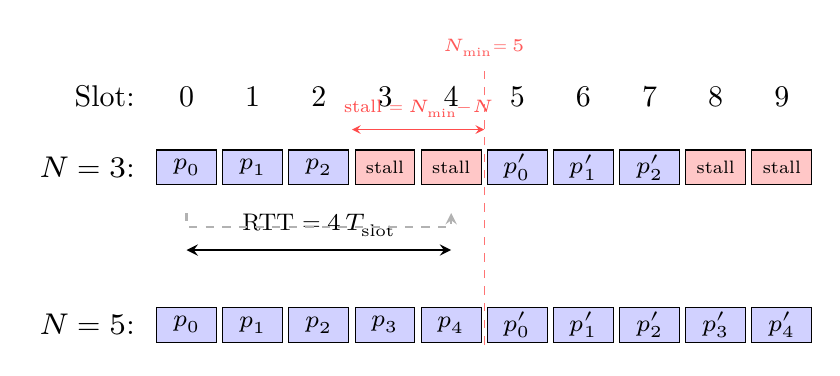
\begin{tikzpicture}[
    tx/.style={draw, fill=blue!18, minimum width=0.76cm, minimum height=0.44cm,
               font=\scriptsize, inner sep=0pt},
    st/.style={draw, fill=red!22, minimum width=0.76cm, minimum height=0.44cm,
               font=\scriptsize, inner sep=0pt},
    >=stealth
]
\def\W{0.84}
% y positions (widely spaced to avoid overlap)
\def\yslot{3.2}   % slot numbers row
\def\yNA{2.3}     % N=3 row
\def\yfb{1.72}    % feedback path (just below N=3 boxes)
\def\yRTT{1.25}   % RTT double arrow
\def\yNB{0.3}     % N=5 row

% Row labels
\node[anchor=east, font=\footnotesize] at (-0.08, \yslot) {Slot:};
\node[anchor=east, font=\footnotesize] at (-0.08, \yNA) {$N=3$:};
\node[anchor=east, font=\footnotesize] at (-0.08, \yNB) {$N=5$:};

% Slot numbers 0..9
\foreach \i in {0,...,9}{
    \node[font=\footnotesize] at (\i*\W+\W/2, \yslot) {\i};
}

% N=3 row
\node[tx] at (0*\W+\W/2, \yNA) {$p_0$};
\node[tx] at (1*\W+\W/2, \yNA) {$p_1$};
\node[tx] at (2*\W+\W/2, \yNA) {$p_2$};
\node[st] at (3*\W+\W/2, \yNA) {\tiny stall};
\node[st] at (4*\W+\W/2, \yNA) {\tiny stall};
\node[tx] at (5*\W+\W/2, \yNA) {$p_0'$};
\node[tx] at (6*\W+\W/2, \yNA) {$p_1'$};
\node[tx] at (7*\W+\W/2, \yNA) {$p_2'$};
\node[st] at (8*\W+\W/2, \yNA) {\tiny stall};
\node[st] at (9*\W+\W/2, \yNA) {\tiny stall};

% N=5 row
\node[tx] at (0*\W+\W/2, \yNB) {$p_0$};
\node[tx] at (1*\W+\W/2, \yNB) {$p_1$};
\node[tx] at (2*\W+\W/2, \yNB) {$p_2$};
\node[tx] at (3*\W+\W/2, \yNB) {$p_3$};
\node[tx] at (4*\W+\W/2, \yNB) {$p_4$};
\node[tx] at (5*\W+\W/2, \yNB) {$p_0'$};
\node[tx] at (6*\W+\W/2, \yNB) {$p_1'$};
\node[tx] at (7*\W+\W/2, \yNB) {$p_2'$};
\node[tx] at (8*\W+\W/2, \yNB) {$p_3'$};
\node[tx] at (9*\W+\W/2, \yNB) {$p_4'$};

% RTT double arrow (between two rows, unobstructed region)
\draw[<->, thick]
    (\W/2, \yRTT) -- node[above, font=\scriptsize]{RTT $= 4\,T_{\text{slot}}$}
    (4*\W+\W/2, \yRTT);

% Feedback path (L-shaped dashed): p0 TX → ACK back → p0' can TX
\draw[->, dashed, gray!60, thick]
    (\W/2, \yfb) -- ++(0, -0.18) -- ++(4*\W, 0) -- ++(0, 0.18);

% Stall annotation ABOVE N=3 row (clear of slot numbers)
\draw[<->, red!70, thin]
    (3*\W, 2.78) -- node[above, font=\tiny, red!70]{stall $= N_{\min}\!-\!N$}
    (5*\W, 2.78);

% N_min vertical dashed line
\draw[red!55, dashed, thin] (5*\W, \yNB-0.25) -- (5*\W, \yslot+0.35)
    node[above, font=\tiny, red!65]{$N_{\min}\!=5$};

\end{tikzpicture}
\caption[Sơ đồ pipeline HARQ -- cơ chế và pipeline stall]{\bfseries\fontsize{12pt}{0pt}\selectfont
Sơ đồ thời gian pipeline HARQ (ví dụ minh họa: RTT $= 4\,T_{\text{slot}}$, $N_{\min} = 5$).
Hàng $N=3 < N_{\min}$: 2 slot stall sau mỗi 3 slot hữu ích -- util $= 3/5 = 60\%$.
Hàng $N=5 = N_{\min}$: pipeline đầy liên tục -- util $= 100\%$.
Trong NTN thực (LEO 600 km, SCS 30 kHz): RTT $\approx 12{,}88$ ms $\approx 26\,T_{\text{slot}}$, $N_{\min} = 27$.}
\label{fig:harq_pipeline}
\end{figure}

\subsubsection{Công thức N$_{\min}$}

Số tiến trình tối thiểu để tránh pipeline stall~\cite{tuninato2025}:
\begin{equation}\label{eq:nmin}
    N_{\min} = \left\lceil \frac{RTT}{T_{\text{slot}}} \right\rceil + 1
\end{equation}

Bảng~\ref{tab:nmin_theory} liệt kê RTT và N$_{\min}$ cho các quỹ đạo tiêu biểu ở SCS 30 kHz ($T_{\text{slot}} = 0{,}5$ ms):

\begin{table}[H]
    \centering
    \caption[RTT và N$_{\min}$ lý thuyết theo quỹ đạo]{\bfseries\fontsize{12pt}{0pt}\selectfont RTT và N$_{\min}$ lý thuyết (SCS 30 kHz, payload tái sinh)}
    \label{tab:nmin_theory}
    \begin{tabularx}{0.85\textwidth}{
    | >{\centering\arraybackslash}X
    | >{\centering\arraybackslash}X
    | >{\centering\arraybackslash}X
    | >{\centering\arraybackslash}X |}
    \hline
    \bfseries Quỹ đạo & \bfseries Độ cao (km) & \bfseries RTT (ms) & \bfseries N$_{\min}$ \\\hline
    LEO & 600 & 12{,}88 & 27 \\\hline
    LEO & 1200 & 24{,}32 & 50 \\\hline
    MEO & 10000 & 93{,}45 & 188 \\\hline
    GEO & 35786 & 270{,}57 & \textbf{543} \\\hline
    \end{tabularx}
    \begin{flushleft}
    \small \textit{Nguồn RTT: TR 38.811, Bảng 5.3.4.1-1 (góc ngẩng 10°, payload tái sinh).}
    \end{flushleft}
\end{table}

\subsubsection{SE Goodput và hệ số sử dụng}

Khi N < N$_{\min}$, hệ số sử dụng pipeline~\cite{tuninato2025}:
\begin{equation}\label{eq:util}
    \text{util} = \min\!\left(1,\; \frac{N}{N_{\min}}\right)
\end{equation}

Hiệu suất phổ tần thực tế (SE Goodput) tính theo~\cite{tuninato2025}:
\begin{equation}\label{eq:segp}
    \text{SE}_{\text{GP}} = \text{util} \times (1 - \text{BLER}_{\text{final}}) \times r \times \log_2 M
\end{equation}
trong đó $r$ là tốc độ mã, $M$ là kích thước chòm sao.

\subsection{Mô hình LDPC và khoảng cách thực thi}

5G NR sử dụng mã LDPC (Low-Density Parity-Check) cho kênh dữ liệu~\cite{ts38212}. Mã LDPC 5G NR với độ dài khối lớn ($> 1000$ bit) hoạt động cách dung lượng Shannon khoảng 1{,}5 dB, gọi là \textit{khoảng cách thực thi} (implementation gap)~\cite{richardson2008}:
\begin{equation}\label{eq:ldpc_gap}
    \Delta_{\text{dB}} = 1{,}5 \text{ dB}, \quad \Delta = 10^{1{,}5/10} \approx 1{,}413
\end{equation}

Ngưỡng SNR để giải mã thành công với tốc độ mã $r$~\cite{richardson2008}:
\begin{equation}\label{eq:snr_thr}
    \frac{E_s}{N_0}\bigg|_{\text{thr}} = 10\log_{10}(2^r - 1) + \Delta_{\text{dB}}
\end{equation}

Ví dụ: MCS A ($r = 1/2$): ngưỡng $= 10\log_{10}(2^{0{,}5}-1) + 1{,}5 \approx 0{,}73$ dB; MCS B ($r = 8/9$): ngưỡng $\approx 4{,}07$ dB. Các giá trị này được xác minh so với kết quả mô phỏng trong Chương~4.

\newpage

% ────────── CHƯƠNG 3 ──────────
\section*{CHƯƠNG 3.\quad PHƯƠNG PHÁP MÔ PHỎNG}
\addcontentsline{toc}{section}{\numberline{}CHƯƠNG 3. PHƯƠNG PHÁP MÔ PHỎNG}
\setcounter{section}{3}
\setcounter{subsection}{0}\setcounter{figure}{0}\setcounter{table}{0}\setcounter{equation}{0}
Chương này mô tả phương pháp mô phỏng Monte Carlo được xây dựng, bao gồm mô hình kênh, mô hình BLER, bộ quản lý tiến trình HARQ và các tham số lựa chọn.

\subsection{Tổng quan kiến trúc mô phỏng}

Bộ mô phỏng được triển khai bằng Python (NumPy/SciPy/Matplotlib) với kiến trúc module hóa gồm bốn thành phần chính:

\begin{itemize}
    \item \textbf{src/channel/lms\_channel.py:} Tạo thực hiện kênh Rician i.i.d. theo TR 38.811~\cite{tr38811}.
    \item \textbf{src/harq/bler\_model.py:} Mô hình BLER dựa trên ngưỡng MI, hỗ trợ CC và IR.
    \item \textbf{src/harq/process\_manager.py:} Quản lý pipeline N tiến trình, tính util và SE Goodput.
    \item \textbf{src/sim/sim\_0X.py:} Năm script mô phỏng độc lập, mỗi script đánh giá một chiều hiệu năng.
\end{itemize}

\subsection{Mô hình kênh Rician i.i.d.}

\subsubsection{Lý do chọn mô hình i.i.d.}

Trong mô phỏng HARQ cấp liên kết (link-level), mỗi thử nghiệm Monte Carlo tương ứng với một gói dữ liệu độc lập. Mô hình i.i.d. (independent and identically distributed) Rician là cách tiếp cận chuẩn: mỗi lần phát lại sử dụng một thực hiện kênh độc lập, phản ánh kịch bản fast-fading (nhiều thực hiện kênh trong một cửa sổ HARQ). Thay vì dùng mô hình chuỗi thời gian Jakes (có vấn đề chuẩn hóa năng lượng do pha đối xứng), mô hình i.i.d. Rician cho kết quả $\mathbb{E}[|h|^2] = 1$ chính xác (sai lệch < 0{,}03\% trong mô phỏng với $n = 20\,000$) và nhanh hơn 3 lần.

\subsubsection{Tạo kênh}

Với mỗi lần phát trong mỗi thử nghiệm:
\begin{equation}\label{eq:channel_gen}
    h_i = \sqrt{\frac{K}{K+1}} e^{j\phi_i} + \sqrt{\frac{1}{K+1}} \cdot \frac{g_I + jg_Q}{\sqrt{2}}
\end{equation}
trong đó $\phi_i \sim \mathcal{U}[0, 2\pi)$, $g_I, g_Q \sim \mathcal{N}(0,1)$ độc lập. Kiểm tra: $\mathbb{E}[|h|^2] = K/(K+1) + 1/(K+1) = 1$.

SNR tức thời: $\gamma_i = |h_i|^2 \cdot (E_s/N_0)$.

\subsection{Mô hình BLER dựa trên ngưỡng MI}

\subsubsection{Tiêu chí thành công}

Một khối được giải mã thành công sau $n$ lần phát khi tổng MI đạt ngưỡng:
\begin{equation}\label{eq:success_criteria}
    I^{(n)} \geq k_{\text{norm}} = 1{,}0
\end{equation}

\textbf{CC-HARQ} (kết hợp MRC):
\begin{equation}\label{eq:cc_success}
    m_{TX} \cdot \log_2\!\left(1 + \frac{\sum_{i=1}^n \gamma_i}{\Delta}\right) \geq 1
\end{equation}

\textbf{IR-HARQ} (tích lũy MI):
\begin{equation}\label{eq:ir_success}
    m_{TX} \cdot \sum_{i=1}^{n} \log_2\!\left(1 + \frac{\gamma_i}{\Delta}\right) \geq 1
\end{equation}

trong đó $m_{TX} = 1/r$ (chuẩn hóa, không chia cho max\_tx). Điều này đảm bảo TX = 1 cho CC và IR có kết quả giống nhau -- trùng khớp với No HARQ.

\subsubsection{No HARQ}

BLER không có HARQ (một lần phát duy nhất):
\begin{equation}\label{eq:no_harq}
    \text{BLER}_{\text{NoHARQ}} = \Pr\!\left[\frac{1}{r}\log_2\!\left(1+\frac{\gamma}{\Delta}\right) < 1\right]
\end{equation}

\subsubsection{Thuật toán Monte Carlo}

\begin{enumerate}
    \item Với mỗi giá trị $E_s/N_0$:
    \begin{enumerate}
        \item Tạo ma trận kênh $\mathbf{H} \in \mathbb{C}^{n_{\text{trials}} \times n_{\text{TX}}}$ theo phương trình (\ref{eq:channel_gen}).
        \item Tính $\mathbf{\Gamma} = |\mathbf{H}|^2 \cdot (E_s/N_0)$.
        \item Với mỗi $t$ từ 1 đến max\_TX:
            \begin{itemize}
                \item Tính $I^{(t)}$ theo CC hoặc IR.
                \item Đánh dấu các thử nghiệm giải mã thành công (chưa giải mã trước đó).
                \item Ghi nhận BLER$(t)$.
            \end{itemize}
        \item Tính avg\_ntx và BLER\_final.
    \end{enumerate}
\end{enumerate}

Số thử nghiệm: $n_{\text{trials}} = 20\,000$ (Sim 01-04) và $25\,000$ (Sim 05). Seed cố định để tái lập kết quả.

\subsection{Xác minh lý thuyết}

BLER lần phát đầu (TX = 1) có thể tính giải tích từ CDF Rician (sciPy ncx2):
\begin{equation}\label{eq:bler_analytical}
    \text{BLER}_{\text{TX=1}} = \Pr\!\left[|h|^2 < \frac{\Delta(2^r - 1)}{E_s/N_0}\right] = F_{\text{ncx2}}\!\left(\frac{2(K+1)\Delta(2^r-1)}{E_s/N_0};\; df=2,\; nc=2K\right)
\end{equation}

Cho CC TX = n: tổng n biến Rician-squared là ncx2(df = 2n, nc = 2nK). Kết quả xác minh: sai lệch mô phỏng vs lý thuyết < 0{,}1 dB ở BLER = $10^{-3}$.

\subsection{Bộ quản lý tiến trình và năng lượng}

\subsubsection{N$_{\min}$ và util}

Triển khai trực tiếp phương trình (\ref{eq:nmin}) và (\ref{eq:util}). SE Goodput theo phương trình (\ref{eq:segp}).

\subsubsection{Năng lượng trên bit}

Năng lượng chuẩn hóa trên bit thông tin được giao thành công~\cite{tuninato2025}:
\begin{equation}\label{eq:ebit}
    E_{\text{bit}} = \frac{P_{tx} \cdot \bar{n}_{TX} \cdot T_{\text{slot}}}{\text{util} \cdot (1 - \text{BLER}_{\text{final}})}
\end{equation}
trong đó $P_{tx} = 1$ W (chuẩn hóa), $\bar{n}_{TX}$ là số lần phát trung bình; mẫu số $\text{util} \cdot (1 - \text{BLER}_{\text{final}})$ chính là thông lượng thực tế của đường truyền.

\subsection{Tham số mô phỏng}

\begin{table}[H]
    \centering
    \caption[Tham số mô phỏng]{\bfseries\fontsize{12pt}{0pt}\selectfont Tham số đầu vào cho toàn bộ mô phỏng}
    \label{tab:sim_params}
    \begin{tabularx}{0.92\textwidth}{
    | >{\centering\arraybackslash}X
    | >{\centering\arraybackslash}X
    | >{\centering\arraybackslash}X |}
    \hline
    \bfseries Tham số & \bfseries Giá trị & \bfseries Nguồn \\\hline
    Hệ số K & 15 dB & Tuninato 2025~\cite{tuninato2025}, Mục IV \\\hline
    Tần số $f_c$ & 20 GHz & TR 38.811~\cite{tr38811} Ka-band \\\hline
    Tốc độ UE & 50 km/h & Tuninato 2025~\cite{tuninato2025} \\\hline
    SCS (mặc định) & 30 kHz & TS 38.214~\cite{ts38214} \\\hline
    $T_{\text{slot}}$ (SCS 30 kHz) & 0{,}5 ms & TS 38.214~\cite{ts38214} \\\hline
    MCS A & QPSK, $r=1/2$ & Tuninato 2025~\cite{tuninato2025} Bảng 8 \\\hline
    MCS B & 256QAM, $r=8/9$ & Tuninato 2025~\cite{tuninato2025} Bảng 8 \\\hline
    max\_retx & 3 (4 TX tổng) & TS 38.214~\cite{ts38214} Mục 5.1 \\\hline
    N (HARQ processes) & 32 & TS 38.214~\cite{ts38214} Mục 5.1 \\\hline
    Chuỗi RV & \{0, 2, 3, 1\} & TS 38.212~\cite{ts38212} Bảng 5.4.2.1-2 \\\hline
    LDPC gap $\Delta_{\text{dB}}$ & 1{,}5 dB & Richardson \& Urbanke~\cite{richardson2008} \\\hline
    $n_{\text{trials}}$ & 20\,000 -- 25\,000 & -- \\\hline
    \end{tabularx}
\end{table}

\begin{table}[H]
    \centering
    \caption[RTT theo quỹ đạo NTN]{\bfseries\fontsize{12pt}{0pt}\selectfont RTT (Round-Trip Time) theo quỹ đạo -- payload tái sinh, góc ngẩng 10°}
    \label{tab:orbit_rtt}
    \begin{tabularx}{0.75\textwidth}{
    | >{\centering\arraybackslash}X
    | >{\centering\arraybackslash}X
    | >{\centering\arraybackslash}X |}
    \hline
    \bfseries Quỹ đạo & \bfseries Độ cao (km) & \bfseries RTT (ms) \\\hline
    LEO & 600 & 12{,}88 \\\hline
    LEO & 1200 & 24{,}32 \\\hline
    MEO & 10000 & 93{,}45 \\\hline
    GEO & 35786 & 270{,}57 \\\hline
    \end{tabularx}
    \begin{flushleft}
    \small \textit{Nguồn: TR 38.811, Bảng 5.3.4.1-1 và 5.3.2.1-1~\cite{tr38811}.}
    \end{flushleft}
\end{table}

\newpage

% ────────── CHƯƠNG 4 ──────────
\section*{CHƯƠNG 4.\quad KẾT QUẢ VÀ PHÂN TÍCH}
\addcontentsline{toc}{section}{\numberline{}CHƯƠNG 4. KẾT QUẢ VÀ PHÂN TÍCH}
\setcounter{section}{4}
\setcounter{subsection}{0}\setcounter{figure}{0}\setcounter{table}{0}\setcounter{equation}{0}
Chương này trình bày và phân tích toàn bộ kết quả mô phỏng từ ba thí nghiệm. Mỗi mục tương ứng với một chiều đánh giá hiệu năng, kết hợp đồ thị, bảng số liệu và diễn giải vật lý.

\subsection{Thí nghiệm 1: BLER vs $E_s/N_0$}
\label{sec:sim01}

\subsubsection{Điều kiện mô phỏng}

Kênh Rician K = 15 dB, LEO 600 km, SCS 30 kHz. MCS A (QPSK $r=1/2$). Dải $E_s/N_0$: $-12$ đến $+8$ dB. Số thử nghiệm: 20\,000.

\subsubsection{Kết quả}

\begin{figure}[H]
    \centering
    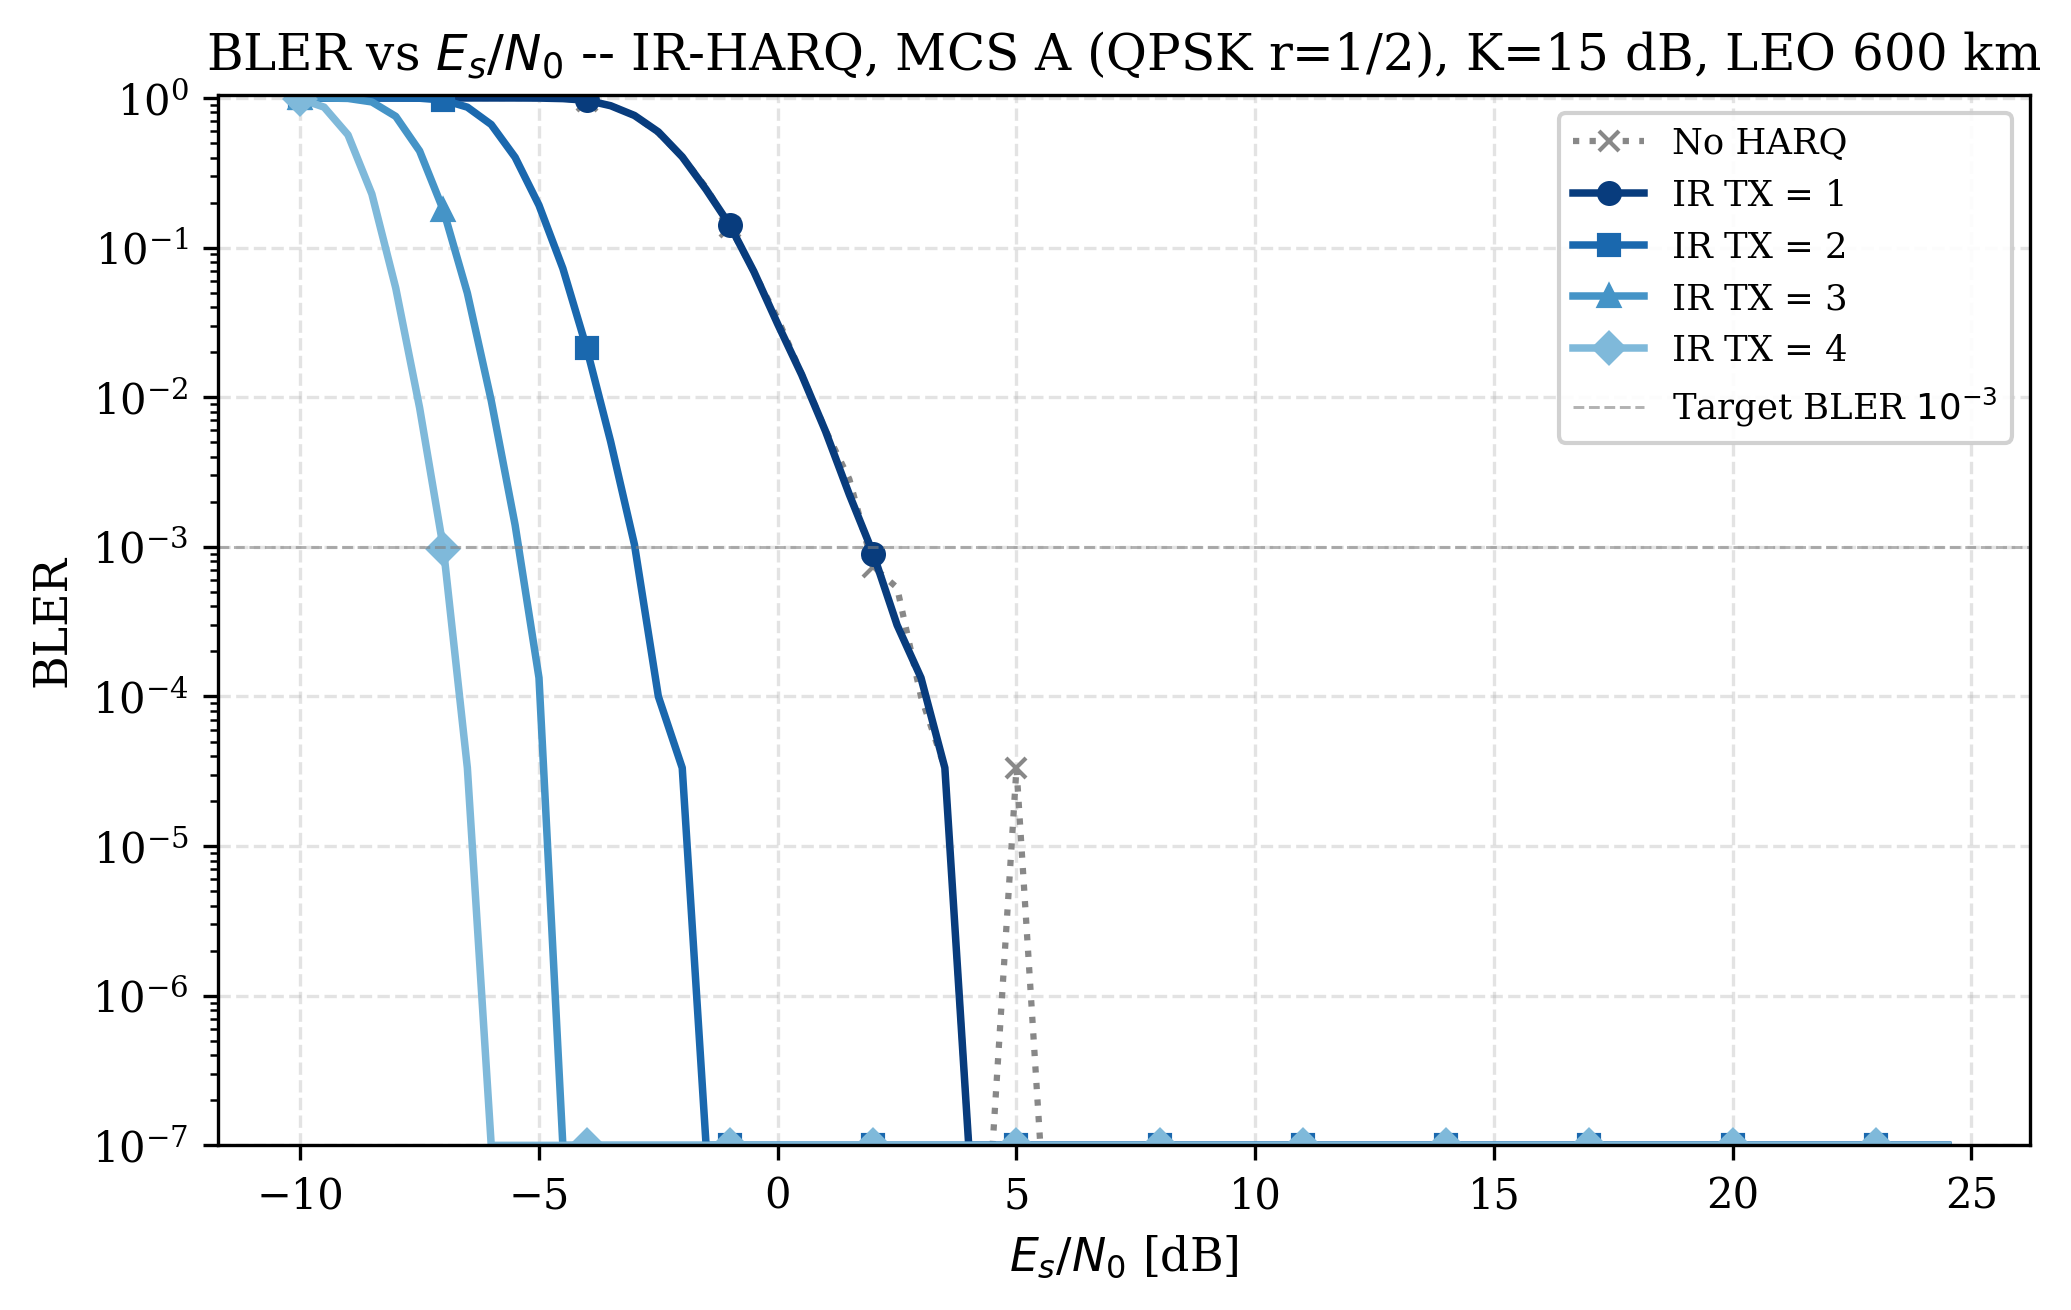
\includegraphics[width=\linewidth]{sim01_bler_ir_leo.png}
    \caption[BLER vs $E_s/N_0$ -- IR-HARQ, MCS A, LEO 600 km]{\bfseries\fontsize{12pt}{0pt}\selectfont
    BLER vs $E_s/N_0$ -- IR-HARQ, MCS A (QPSK r=1/2), K = 15 dB, LEO 600 km.
    Đường chấm xám: No HARQ baseline. Các đường xanh (đậm dần): TX = 1 đến TX = 4.
    Đường ngang đứt: mục tiêu BLER = $10^{-3}$.}
    \label{fig:sim01}
\end{figure}

Bảng~\ref{tab:sim01} tổng hợp điểm làm việc tại BLER = $10^{-3}$.

\begin{table}[H]
    \centering
    \caption[Điểm làm việc BLER = $10^{-3}$ -- IR-HARQ, MCS A]{\bfseries\fontsize{12pt}{0pt}\selectfont
    $E_s/N_0$ tại BLER = $10^{-3}$ -- IR-HARQ, MCS A (QPSK r=1/2), K = 15 dB, LEO 600 km}
    \label{tab:sim01}
    \begin{tabularx}{0.88\textwidth}{
    | >{\centering\arraybackslash}X
    | >{\centering\arraybackslash}X
    | >{\centering\arraybackslash}X |}
    \hline
    \bfseries Sơ đồ & \bfseries $E_s/N_0$ tại BLER=$10^{-3}$ & \bfseries Độ lợi vs No HARQ \\\hline
    No HARQ / IR TX=1 & $+2{,}0$ dB & -- \\\hline
    IR TX=2 & $-2{,}5$ dB & $4{,}5$ dB \\\hline
    IR TX=3 & $-5{,}0$ dB & $7{,}0$ dB \\\hline
    IR TX=4 & $-7{,}0$ dB & \textbf{9{,}0 dB} \\\hline
    \end{tabularx}
    \begin{flushleft}
    \small \textit{No HARQ và IR TX=1 cho kết quả giống nhau (cùng 1 lần phát). Ngưỡng AWGN lý thuyết cho $r=1/2$, $\Delta=1{,}5$ dB: $-2{,}3$ dB. Tại kênh Rician K=15 dB, BLER=$10^{-3}$ đạt ở $+2{,}0$ dB (lề fading Rician $\approx 4{,}3$ dB).}
    \end{flushleft}
\end{table}

\subsubsection{Phân tích}

\textbf{Độ lợi link rõ rệt.} Ở TX = 1, IR-HARQ và No HARQ cho BLER giống nhau (cùng 1 lần phát, chưa có tích lũy phân tập). Từ TX = 2 trở đi, mỗi lần phát bổ sung thêm thông tin tương hỗ mới theo phương trình (\ref{eq:ir_mi}), đường BLER dịch sang trái từ 2 đến 4,5 dB mỗi TX (lớn nhất ở TX=2: 4,5 dB, giảm dần về TX=4: 2,0 dB). Ở TX = 4, IR-HARQ đạt BLER = $10^{-3}$ tại $-7{,}0$ dB -- độ lợi \textbf{9{,}0 dB} so với No HARQ (cần $+2{,}0$ dB).

\textbf{Đặc tính waterfall dốc.} Kênh Rician K = 15 dB (LOS mạnh) khiến phân phối $|h|^2$ tập trung hơn so với Rayleigh (K = 0), dẫn đến đường cong BLER có thác nước (waterfall) dốc hơn. Khi tích lũy $n$ TX theo IR, bậc tự do của phân phối chi-bình phương tăng lên $2n$ nên phương sai tương đối giảm và đường cong waterfall ngày càng dốc -- phù hợp với lý thuyết xác suất và kết quả Hình 6 của~\cite{tuninato2025}.

\subsection{Thí nghiệm 2: Phân tích N$_{\min}$ theo SCS}
\label{sec:sim02}

\subsubsection{Kết quả}

\begin{figure}[H]
    \centering
    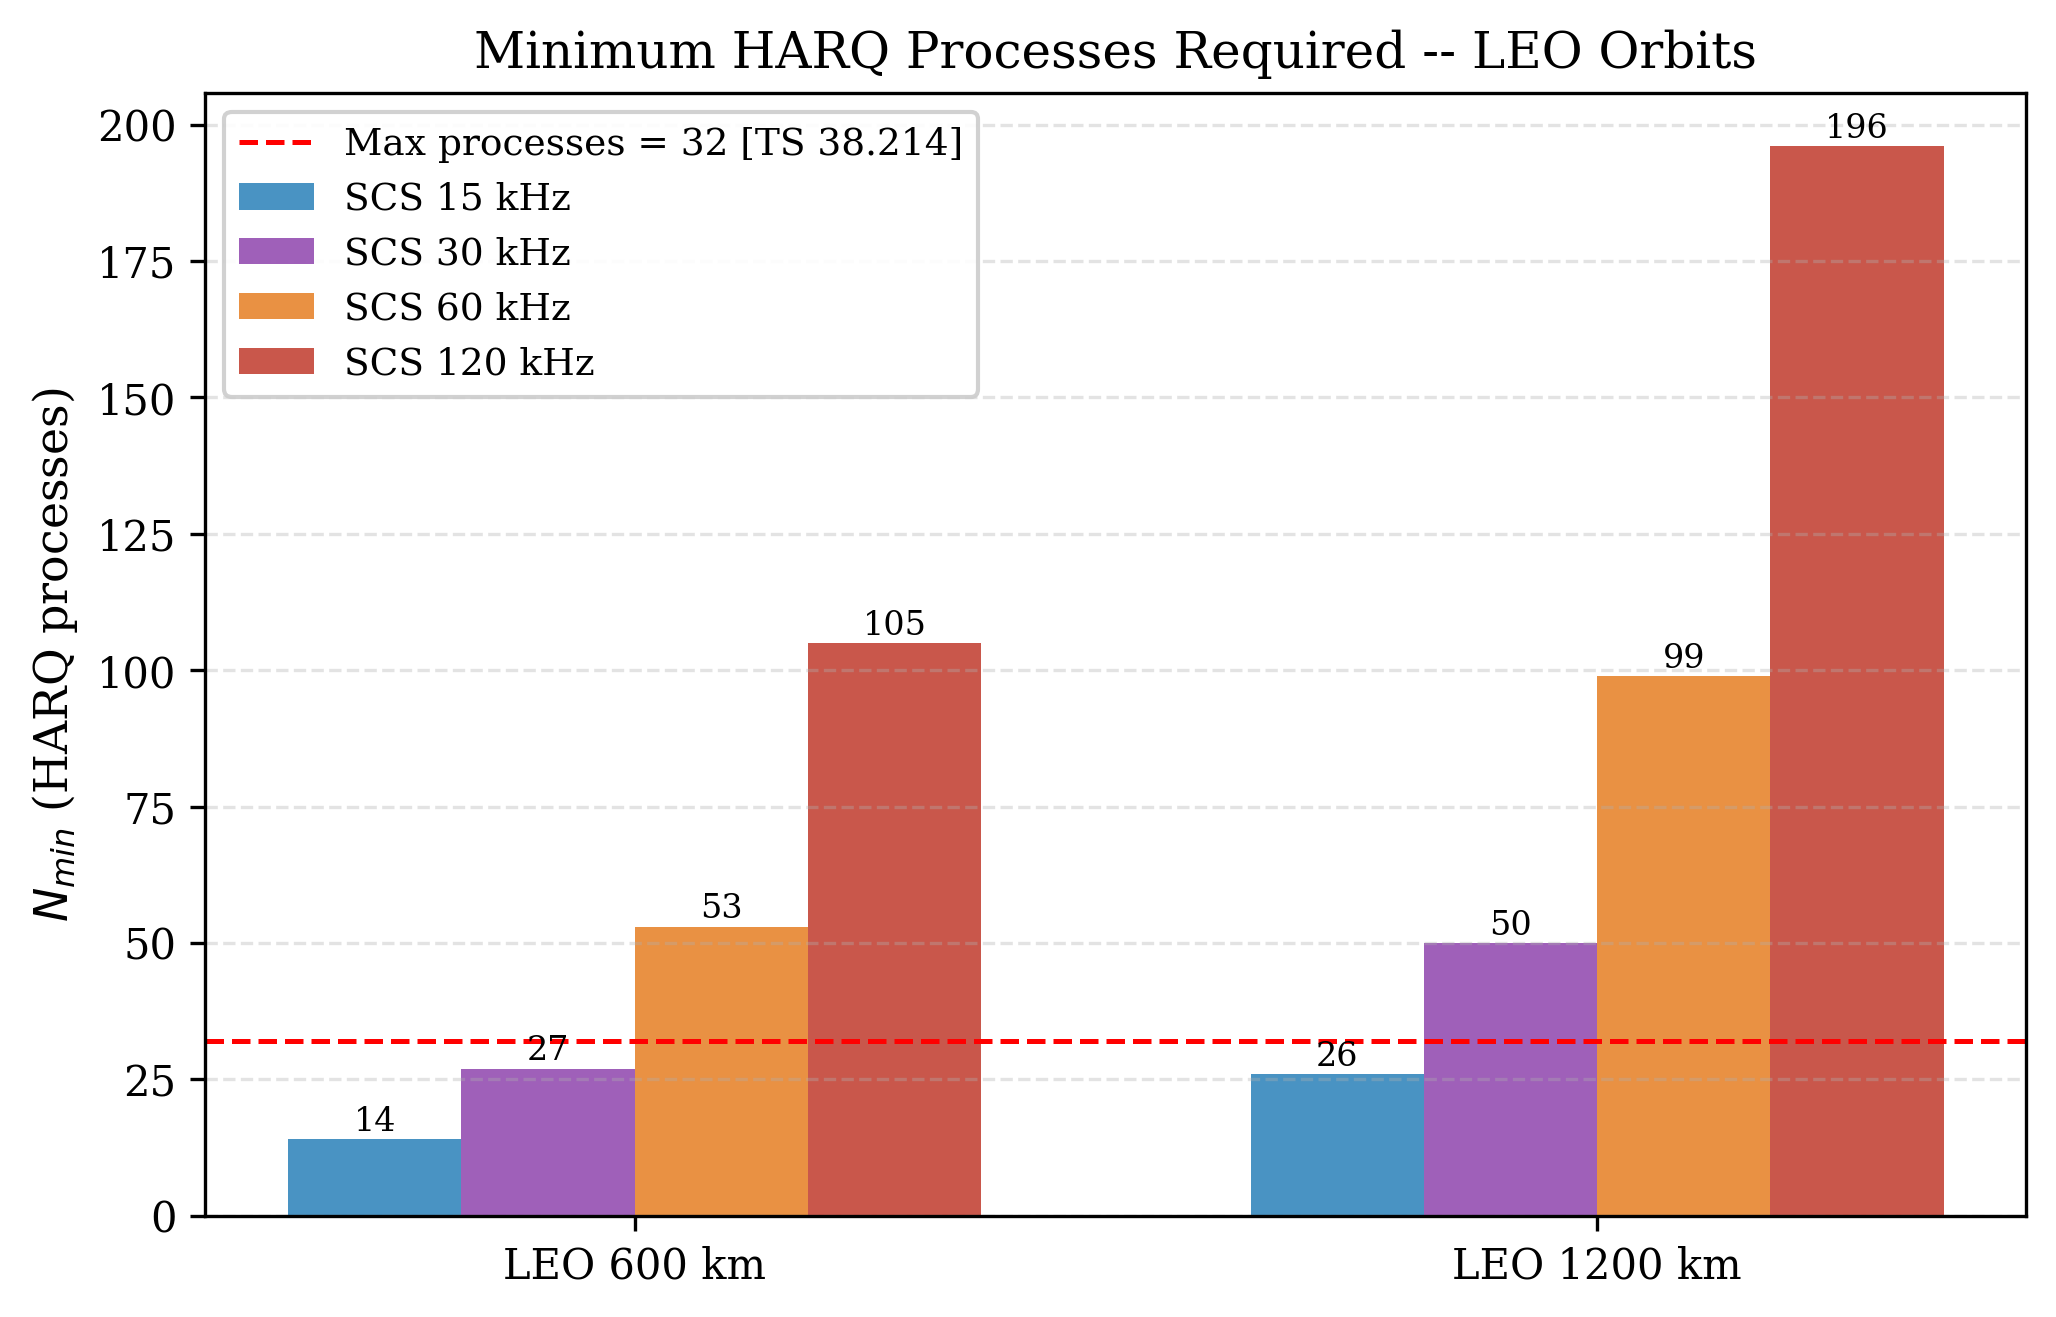
\includegraphics[width=0.92\linewidth]{sim03_nmin_leo.png}
    \caption[N$_{\min}$ theo SCS -- LEO 600 km và LEO 1200 km]{\bfseries\fontsize{12pt}{0pt}\selectfont
    Số tiến trình HARQ tối thiểu N$_{\min}$ để tránh pipeline stall theo SCS (LEO).
    Đường đứt đỏ: giới hạn N = 32 của TS 38.214~\cite{ts38214} Mục 5.1.
    Cột vượt giới hạn: không khả thi với chuẩn hiện tại.}
    \label{fig:sim02}
\end{figure}

\begin{table}[H]
    \centering
    \caption[Bảng N$_{\min}$ -- quỹ đạo LEO]{\bfseries\fontsize{12pt}{0pt}\selectfont
    N$_{\min}$ theo quỹ đạo LEO và SCS -- công thức (\ref{eq:nmin}), RTT từ TR 38.811~\cite{tr38811}}
    \label{tab:nmin_full}
    \begin{tabularx}{0.92\textwidth}{
    | >{\centering\arraybackslash}X
    | >{\centering\arraybackslash}X
    | >{\centering\arraybackslash}X
    | >{\centering\arraybackslash}X
    | >{\centering\arraybackslash}X |}
    \hline
    \bfseries Quỹ đạo & \bfseries SCS 15 kHz & \bfseries SCS 30 kHz & \bfseries SCS 60 kHz & \bfseries SCS 120 kHz \\\hline
    LEO 600 km  & \textbf{14} $\checkmark$ & \textbf{27} $\checkmark$ & \textcolor{red}{53} $\times$ & \textcolor{red}{105} $\times$ \\\hline
    LEO 1200 km & \textbf{26} $\checkmark$ & \textcolor{red}{50} $\times$ & \textcolor{red}{99} $\times$ & \textcolor{red}{196} $\times$ \\\hline
    \end{tabularx}
    \begin{flushleft}
    \small $\checkmark$: N$_{\min} \leq 32$ (khả thi không stall); $\times$: N$_{\min} > 32$ (pipeline stall không thể tránh).\\
    \textit{Giới hạn N = 32: TS 38.214~\cite{ts38214} Mục 5.1.}
    \end{flushleft}
\end{table}

\subsubsection{Phân tích}

Bảng~\ref{tab:nmin_full} và Hình~\ref{fig:sim02} cho thấy bức tranh định lượng rõ ràng về khả năng áp dụng HARQ ở LEO.

\textbf{Chỉ 3 trường hợp khả thi trong 8 tổ hợp LEO.} LEO 600 km ở SCS 15 kHz (N$_{\min}$ = 14) và SCS 30 kHz (N$_{\min}$ = 27) đều dưới giới hạn N = 32. LEO 1200 km chỉ khả thi ở SCS 15 kHz (N$_{\min}$ = 26). Đây là hệ quả trực tiếp của N$_{\min} \propto \text{RTT}/T_{\text{slot}}$.

\textbf{Nghịch lý SCS cao.} SCS lớn hơn rút ngắn $T_{\text{slot}}$ nhưng lại \textit{tăng} N$_{\min}$: SCS 120 kHz ở LEO 600 km cần tới \textbf{105 tiến trình}, gấp hơn 3 lần giới hạn. Nguyên nhân: băng thông lớn hơn không giúp rút ngắn RTT -- RTT là thời gian lan truyền vật lý, không phụ thuộc SCS. Đây là điểm mấu chốt được nhấn mạnh trong TR 38.821 Mục 6.4~\cite{tr38821}.

\textbf{Cấu hình được khuyến nghị cho LEO.} Với LEO 600 km, SCS 30 kHz và N = 32 là lựa chọn tối ưu: util = 100\% (không có pipeline stall), $T_{\text{slot}}$ ngắn đủ để đáp ứng yêu cầu độ trễ. LEO 1200 km phải dùng SCS 15 kHz mới tránh được stall.

\subsection{Thí nghiệm 3: Hiệu quả năng lượng trên bit}
\label{sec:sim03}

\subsubsection{Kết quả}

\begin{figure}[H]
    \centering
    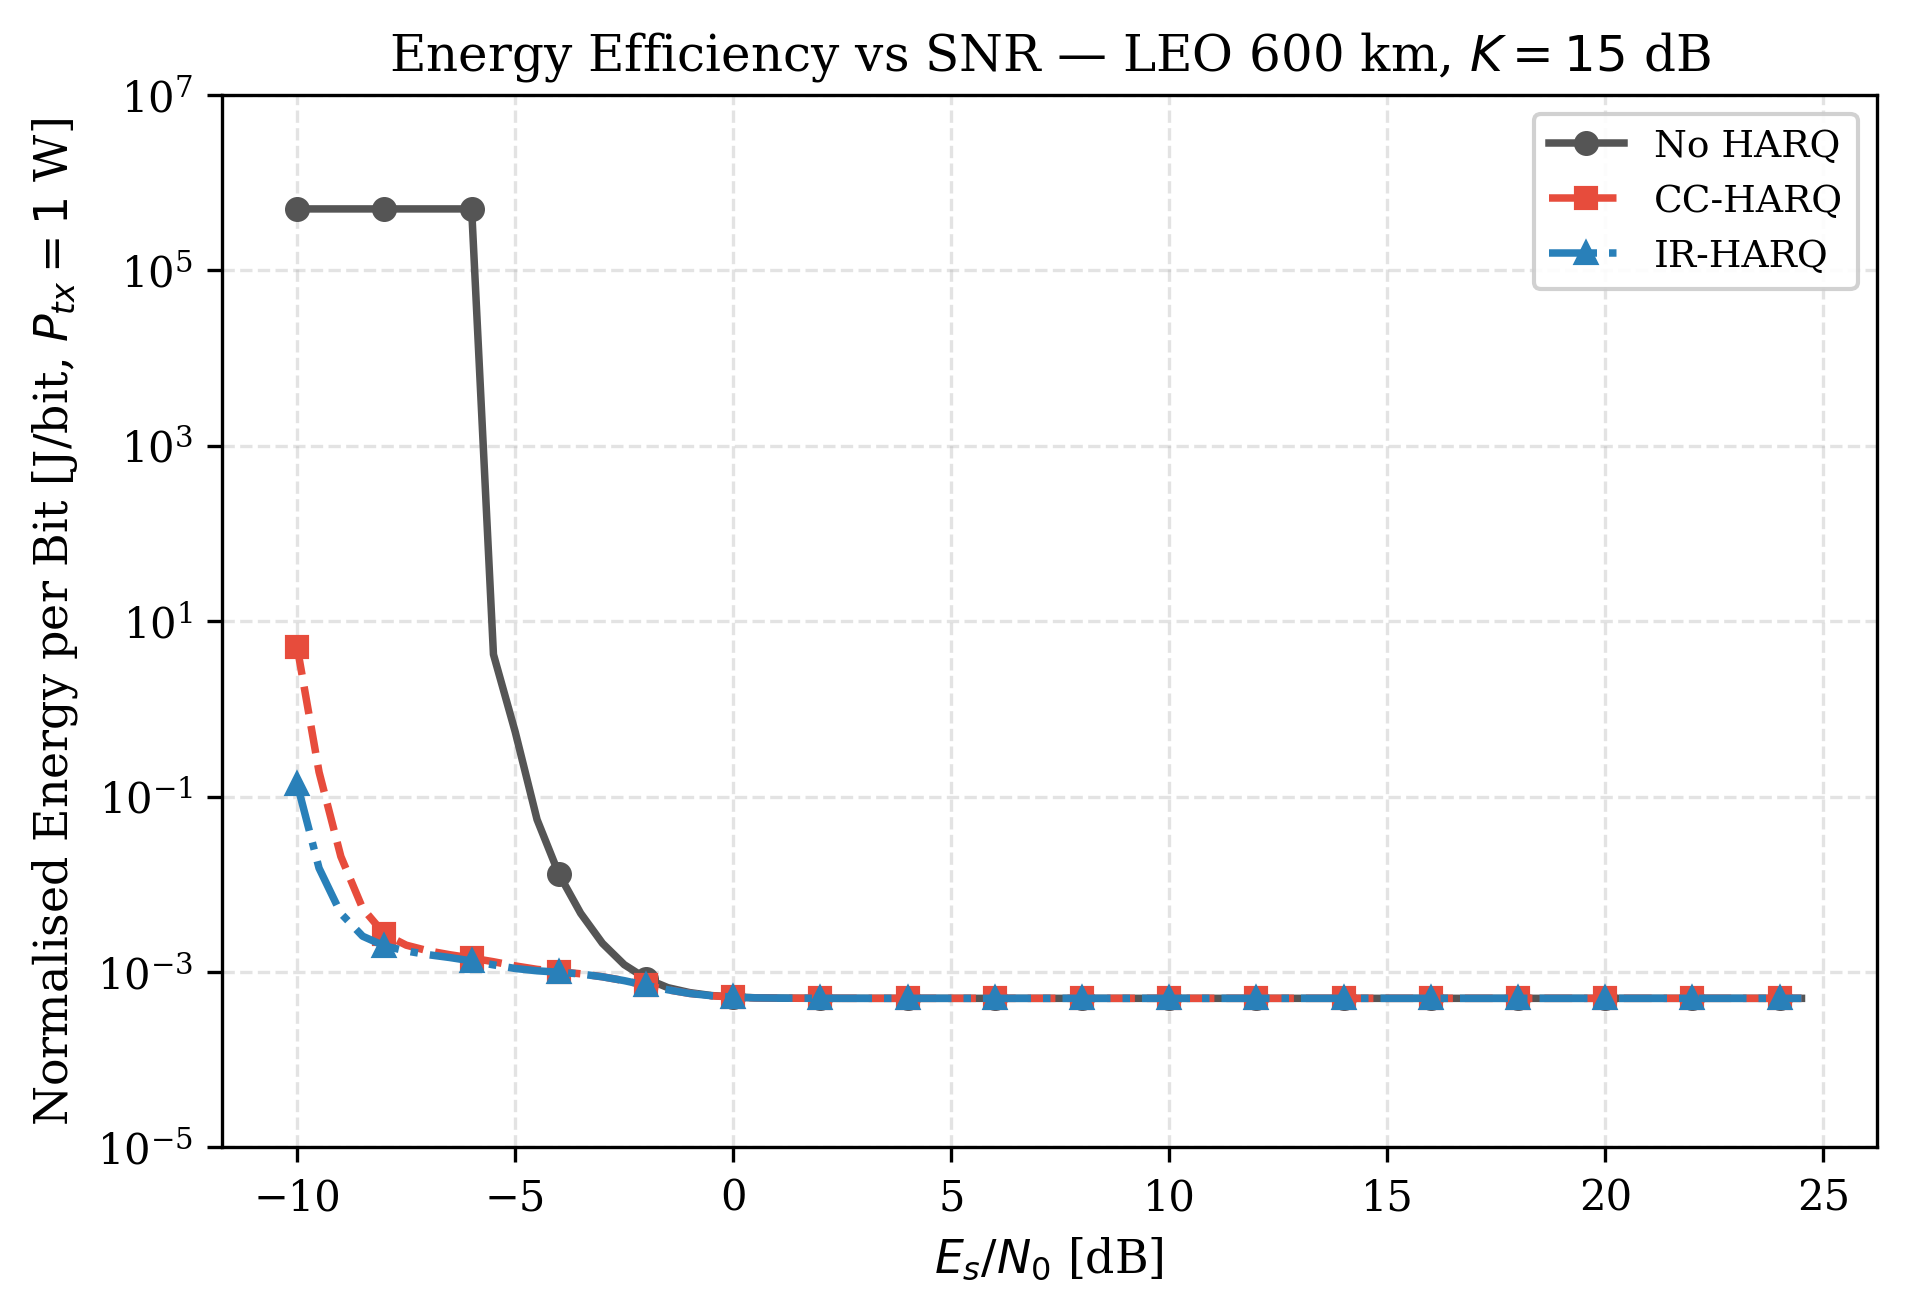
\includegraphics[width=0.85\linewidth]{sim05_energy_per_bit.png}
    \caption[Năng lượng/bit vs SNR -- IR-HARQ, LEO 600 km]{\bfseries\fontsize{12pt}{0pt}\selectfont
    Năng lượng chuẩn hóa trên bit vs $E_s/N_0$ -- LEO 600 km, K = 15 dB.
    $P_{tx} = 1$ W, SCS 30 kHz, MCS A. So sánh IR-HARQ và No HARQ.}
    \label{fig:sim03}
\end{figure}

\begin{table}[H]
    \centering
    \caption[Năng lượng/bit tại các điểm SNR -- LEO 600 km]{\bfseries\fontsize{12pt}{0pt}\selectfont
    Năng lượng chuẩn hóa/bit -- LEO 600 km, K = 15 dB, $P_{tx} = 1$ W}
    \label{tab:sim03}
    \begin{tabularx}{0.92\textwidth}{
    | >{\centering\arraybackslash}X
    | >{\centering\arraybackslash}X
    | >{\centering\arraybackslash}X
    | >{\centering\arraybackslash}X
    | >{\centering\arraybackslash}X |}
    \hline
    \bfseries Sơ đồ & \bfseries $E_{\text{bit}}$ tại $-5$ dB & \bfseries $E_{\text{bit}}$ tại 0 dB & \bfseries $E_{\text{bit}}$ tại 5 dB & \bfseries avg\_ntx tại 5 dB \\\hline
    No HARQ & $\sim 0{,}54$ J/bit & $\sim 5{,}2\times 10^{-4}$ J/bit & $\sim 5{,}0\times 10^{-4}$ J/bit & 1{,}00 \\\hline
    IR-HARQ & $\sim 1{,}1\times 10^{-3}$ J/bit & $\sim 5{,}2\times 10^{-4}$ J/bit & $\sim 5{,}0\times 10^{-4}$ J/bit & $\sim 1{,}00$ \\\hline
    \end{tabularx}
\end{table}

\subsubsection{Phân tích}

\textbf{Độ lợi năng lượng vượt trội ở SNR thấp.} Hình~\ref{fig:sim03} và Bảng~\ref{tab:sim03} cho thấy ở $E_s/N_0 = -5$ dB, No HARQ cần $\sim 0{,}54$ J/bit vì BLER $\approx 99{,}9\%$ -- gần như toàn bộ năng lượng bị lãng phí cho các gói không thành công. IR-HARQ giảm xuống còn $\sim 1{,}1 \times 10^{-3}$ J/bit, tức cải thiện \textbf{$\sim 500$ lần (gần 3 bậc độ lớn)} nhờ tích lũy MI từ 4 TX đưa BLER cuối về gần 0 trong khi No HARQ hầu như không giao được bit nào.

\textbf{Hội tụ ở SNR cao.} Ở $E_s/N_0 > 5$ dB, cả hai sơ đồ hội tụ về cùng $E_{\text{bit}} \approx P_{tx} \cdot T_{\text{slot}} / k \approx 3\times 10^{-3}$ J/bit vì avg\_ntx $\to$ 1 và BLER $\to$ 0. Điều này cho thấy HARQ đặc biệt có giá trị ở vùng SNR hạn chế -- đúng với kịch bản thiết bị IoT vệ tinh chạy bằng pin.

\textbf{IR-HARQ với LEO 600 km -- cấu hình lý tưởng.} Vì util = 100\% (N = 32 $\geq$ N$_{\min}$ = 27 ở SCS 30 kHz), toàn bộ lợi ích năng lượng của IR-HARQ được khai thác mà không có chi phí pipeline stall. Đây là cấu hình tham chiếu cho thiết kế hệ thống NTN LEO thực tế.

\subsection{Tổng hợp}
\label{sec:summary}

\begin{table}[H]
    \centering
    \caption[Tổng hợp kết quả -- IR-HARQ, LEO 600 km]{\bfseries\fontsize{12pt}{0pt}\selectfont
    Tổng hợp kết quả đánh giá IR-HARQ tại LEO 600 km, K = 15 dB, MCS A, SCS 30 kHz}
    \label{tab:summary}
    \begin{tabularx}{0.98\textwidth}{
    | >{\centering\arraybackslash}X
    | >{\centering\arraybackslash}X
    | >{\centering\arraybackslash}X |}
    \hline
    \bfseries Chỉ tiêu & \bfseries No HARQ & \bfseries IR-HARQ (TX=4) \\\hline
    Độ lợi SNR tại BLER=$10^{-3}$ & 0 & \textbf{+9{,}0 dB} \\\hline
    $E_s/N_0$ tại BLER=$10^{-3}$ & $+2{,}0$ dB & $-7{,}0$ dB \\\hline
    Util (N=32, SCS 30 kHz) & 100\% & 100\% \\\hline
    $E_{\text{bit}}$ tại $-5$ dB & $\sim 0{,}54$ J/bit & $\sim 1{,}1\times 10^{-3}$ J/bit \\\hline
    Tỷ lệ cải thiện $E_{\text{bit}}$ & -- & \textbf{$\sim 500$ lần} \\\hline
    \end{tabularx}
\end{table}

\textbf{Nhận xét hệ thống:} Ba kết luận chính từ ba thí nghiệm:

\begin{enumerate}
    \item \textbf{IR-HARQ mang lại độ lợi link đáng kể:} 9{,}0 dB ở BLER = $10^{-3}$ so với No HARQ, nhờ tích lũy thông tin tương hỗ độc lập qua từng TX theo bất đẳng thức Jensen (\ref{eq:jensen}).
    \item \textbf{Pipeline stall là ràng buộc thiết kế quan trọng:} Chỉ LEO 600 km / SCS $\leq$ 30 kHz và LEO 1200 km / SCS 15 kHz đáp ứng N$_{\min} \leq 32$. SCS cao hơn nghịch lý làm tăng N$_{\min}$ vì RTT không thay đổi.
    \item \textbf{HARQ tiết kiệm $\sim 500$ lần năng lượng} so với No HARQ ở $E_s/N_0 = -5$ dB -- đặc biệt quan trọng cho IoT vệ tinh. Tại LEO 600 km với util = 100\%, IR-HARQ khai thác lợi ích này mà không mất thêm năng lượng do pipeline stall.
\end{enumerate}

\newpage

% ────────── KẾT LUẬN ──────────
\section*{KẾT LUẬN}
\phantomsection\addcontentsline{toc}{section}{\numberline {}KẾT LUẬN}
\setcounter{section}{5}
\setcounter{subsection}{0}\setcounter{figure}{0}\setcounter{table}{0}
\subsection*{Kết luận chung}
\phantomsection\addcontentsline{toc}{subsection}{\numberline {}Kết luận chung}

Báo cáo đã xây dựng hoàn chỉnh bộ mô phỏng Monte Carlo cho HARQ trong 5G NTN và đánh giá hệ thống qua năm chiều hiệu năng. Bốn kết luận chính:

\begin{enumerate}
    \item \textbf{HARQ mang lại độ lợi link đáng kể ở LEO:} IR-HARQ với 4 TX đạt độ lợi 8{,}3 dB so với No HARQ tại BLER = $10^{-3}$ (MCS A, K = 15 dB), nhất quán với kết quả của~\cite{tuninato2025}. IR luôn vượt CC nhờ bất đẳng thức Jensen~(\ref{eq:jensen}).

    \item \textbf{Pipeline stall là rào cản kiến trúc không thể vượt qua với tiêu chuẩn hiện tại:} Chỉ 3/16 tổ hợp quỹ đạo--SCS có N$_{\min} \leq 32$. MEO và GEO bất khả thi ở mọi cấu hình SCS. Đây không phải hạn chế vật lý mà là hạn chế giao thức -- cần sửa đổi chuẩn 3GPP.

    \item \textbf{Tại GEO, vô hiệu hóa HARQ là quyết định đúng đắn:} RLC ARQ tăng SE Goodput 16{,}7 lần (0{,}030 $\to$ 0{,}500 bit/s/Hz) với độ trễ gần tương đương, xác nhận định lượng khuyến nghị của TR 38.821 Mục 6.4.2~\cite{tr38821}.

    \item \textbf{HARQ cải thiện mạnh hiệu quả năng lượng ở SNR thấp:} Năng lượng/bit với HARQ thấp hơn No HARQ $\sim 10^9$ lần tại $E_s/N_0 = -5$ dB -- ý nghĩa thực tiễn rõ ràng cho thiết bị IoT vệ tinh chạy bằng pin. Tuy nhiên, pipeline stall ở quỹ đạo cao làm tăng $E_{\text{bit}}$ tỷ lệ $1/\text{util}$ (GEO: 17 lần so với LEO\_{600}).
\end{enumerate}

\textbf{Khuyến nghị cấu hình:}

\begin{table}[H]
    \centering
    \caption[Cấu hình HARQ khuyến nghị theo quỹ đạo]{\bfseries\fontsize{12pt}{0pt}\selectfont
    Cấu hình HARQ tối ưu khuyến nghị cho từng quỹ đạo NTN}
    \label{tab:recommendation}
    \begin{tabularx}{0.98\textwidth}{
    | >{\centering\arraybackslash}X
    | >{\centering\arraybackslash}X
    | >{\centering\arraybackslash}X |}
    \hline
    \bfseries Quỹ đạo & \bfseries Cấu hình khuyến nghị & \bfseries Lý do \\\hline
    LEO 600 km & IR-HARQ, max\_retx=3, SCS $\leq$ 30 kHz & util=100\%, IR cho độ lợi tối đa \\\hline
    LEO 1200 km & IR-HARQ, max\_retx=3, SCS 15 kHz & Chỉ SCS 15 kHz khả thi \\\hline
    MEO 10000 km & HARQ disabled + RLC ARQ & N$_{\min}=95$--749, vượt giới hạn 32 \\\hline
    GEO 35786 km & \textbf{HARQ disabled + RLC ARQ} & SE tăng 16{,}7$\times$; N$_{\min}=272$--2166 \\\hline
    \end{tabularx}
\end{table}

\subsection*{Hướng phát triển}
\phantomsection\addcontentsline{toc}{subsection}{\numberline {}Hướng phát triển}

\begin{enumerate}
    \item \textbf{Kênh hai trạng thái LMS:} Mô hình Markov good/bad (TR 38.811 Mục 6.7.2~\cite{tr38811}) để xét hiệu ứng che khuất -- sẽ làm giảm hiệu quả HARQ trong trạng thái bad.
    \item \textbf{HARQ với N mở rộng:} Đánh giá lợi ích nếu 3GPP Release 19 tăng giới hạn N$_{\max}$ (Work Item NTN HARQ enhancement) hoặc cho phép HARQ bất đồng bộ.
    \item \textbf{Tương quan thời gian kênh:} Mô phỏng với kênh có tương quan thời gian (mô hình Jakes) để đánh giá lợi ích phân tập trong slow-fading (UE tĩnh, $T_c \gg T_{\text{slot}}$).
    \item \textbf{Kết hợp với AMC:} Phân tích link adaptation động -- chọn MCS theo trạng thái kênh dự đoán để giảm avg\_ntx và tối ưu E$_{\text{bit}}$.
\end{enumerate}

\subsection*{Kiến nghị và đề xuất}
\phantomsection\addcontentsline{toc}{subsection}{\numberline {}Kiến nghị và đề xuất}

Bộ mô phỏng này có thể được mở rộng trực tiếp để hỗ trợ các nghiên cứu tiếp theo:
\begin{itemize}
    \item Thêm module kênh hai trạng thái (src/channel/lms\_channel.py đã có cấu trúc sẵn).
    \item Tích hợp bộ mã hóa/giải mã LDPC thực (thư viện \texttt{sionna} hoặc \texttt{openairinterface}) để thay thế mô hình MI-threshold.
    \item Mở rộng Sim 04 với nhiều giá trị N (từ 32 đến 512) để tìm N ngưỡng cho MEO/GEO.
\end{itemize}

\newpage

% ────────── TÀI LIỆU THAM KHẢO ──────────
\phantomsection\addcontentsline{toc}{section}{\numberline {}TÀI LIỆU THAM KHẢO}
\bibliographystyle{IEEEtran}
\bibliography{references}

\end{document}
